%!TEX root = pcp.tex

\subsection{Models comparison}

We executed a test suite for determining which inequalities to use in the formulation of the problem. Recall from section \ref{sec:model} that there are several restrictions that can be applied to define the model, as well as additional ones that may strengthen the model or reduce the number of symmetrical solutions.

In order to test the effectiveness of the different formulations, we applied a fixed number of cutting planes iterations, using all implemented cuts with a slightly aggressive configuration, and reported the resulting MIP gap and running time (in seconds), as well as how many rounds of cutting planes were executed. It is worth noting that in some cases fewer iterations than total were applied as the separation heuristics were not able to find any more violated inequalities.

For these tests we used binomial graphs with a fixed size of 100 nodes with exactly 2 nodes per partition, and powerlaw cluster graphs with the same size, changing only the density of the graphs. All graphs were preprocessed beforehand.

\subsubsection{Adjacency constraints}

We first tested the four different adjacency (or color conflict) constraints we had proposed, using arbitrarily chosen constraints \ref{eqn:partsum}, \ref{eqn:lowerlabel} and \ref{eqn:wjleqsumcolor} to complete the model:

\begin{align*}
&\sum_{i \in P_k} \sum_{j \in C} x_{ij} = 1 &\quad \forall P_k \in P \tag{\ref{eqn:partsum}} \\
&w_j \geq w_{j+1} &\quad \forall 1 \leq j < c \tag{\ref{eqn:lowerlabel}} \\
&w_j \leq \sum_{i \in V} x_{ij} &\quad \forall j \in C \tag{\ref{eqn:wjleqsumcolor}} \\
\end{align*}

The different adjacency constraints being tested in this experiment are the following: 

\begin{align*}
&x_{ij} + x_{kj} \leq w_j \sumheight &\quad \forall (i,k) \in E, \; \forall j \in C \tag{\ref{eqn:adjscolorp}} \\
&x_{ij} + x_{kj} \leq 1 \sumheight &\quad \forall (i,k) \in E, \; \forall j \in C \tag{\ref{eqn:adjscolorpone}} \\
&\sum_{i \in N(i_0)} x_{i_0j} + r * x_{i_0j} \leq r * w_j &\quad \forall j \in C, \; \forall i_0 \in V \tag{\ref{eqn:adjsneighb}} \\
&\sum_{i \in P_k \cap N(i_0)} x_{ij} + x_{i_0j} \leq w_j &\quad \forall j \in C, \; \forall P_k \in P, \; \forall i_0 \in V \tag{\ref{eqn:adjsperpart}} 
\end{align*}

Results are displayed on table \ref{table:modelsadj}. Differences between gaps are almost non existent, whereas time required changes greatly between graphs with different densities. On higher density graphs, constraints \ref{eqn:adjsneighb} using a clique coverage of the neighbourhood report a better running time than the others; while on lower density \ref{eqn:adjscolorpone} works better than \ref{eqn:adjscolorp}, even though the former uses $n \times c$ additional constraints \ref{eqn:nodelessthanwj}.

\begin{sidewaystable}
\centering

	\begin{tabular}{|c|ccc|ccc|ccc|ccc|}
	\hline
	\multicolumn{1}{|c|}{Id} & \multicolumn{3}{|c|}{Constraint \ref{eqn:adjscolorp}} & \multicolumn{3}{|c|}{Constraint \ref{eqn:adjscolorpone}} & \multicolumn{3}{|c|}{Constraint \ref{eqn:adjsneighb}} & \multicolumn{3}{|c|}{Constraint \ref{eqn:adjsperpart}} 
	\\
	& gap & rounds & time & gap & rounds & time & gap & rounds & time & gap & rounds & time 
	\\
	\hline
	EW 20\% & 0.458 & 14.6 & 5.632 & 0.458 & 10.6 & \b{4.568} & 0.458 & 20.4 & 7.915 & 0.458 & 16.2 & 5.728
	\\
	EW 40\% & 0.466 & 22.4 & 16.998 & 0.466 & 25.6 & \b{14.09} & 0.466 & 32.6 & 17.884 & 0.466 & 24.8 & 16.976
	\\
	EW 60\% & 0.42 & 62.8 & 98.642 & 0.42 & 57.4 & \b{77.694} & 0.42 & 72.6 & 87.575 & 0.42 & 78.6 & 120.138
	\\
	EW 80\% & 0.292 & 193.0 & 449.054 & 0.296 & 181.2 & 469.844 & 0.292 & 192.4 & \b{349.557} & 0.294 & 160.0 & 451.126
	\\
	\hline
	HK 10\% &  0.2 &  0.8 & 0.156 &  0.2 &  0.8 & 0.128 &  0.2 &  0.8 & 0.106 &  0.2 &  0.8 & 0.168
	\\
	HK 20\% & 0.12 &  0.6 & 0.278 & 0.12 &  0.6 & 0.324 &  0.2 &  1.0 & 0.181 & 0.12 &  0.6 & 0.306
	\\
	HK 30\% &  0.0 &  0.8 & 0.308 &  0.0 &  0.8 & 0.276 &  0.0 &  3.2 & 0.489 &  0.0 &  0.8 & 0.318
	\\
	HK 40\% & 0.048 &  2.2 & 0.28 & 0.048 &  3.0 & 0.312 & 0.048 &  5.2 & 0.416 & 0.048 &  2.6 & 0.292
	\\
	\hline 
	 \end{tabular}
	
	\caption{Comparison of different color conflict constraints on the model formulation: adjacent nodes sum bounded by $w_j$ (\ref{eqn:adjscolorp}), adjacent nodes sum bounded by $1$ (\ref{eqn:adjscolorpone}), adjacencies grouped by partition (\ref{eqn:adjsperpart}) and using clique coverage of the neighbourhood (\ref{eqn:adjsneighb}).}
	\label{table:modelsadj}
\end{sidewaystable}

\subsubsection{Colored nodes per partition}

A quick test we also ran in parallel was to determine whether to paint exactly one node per partition (\ref{eqn:partsum}), or to relax this constraint and allow for painting more than a single node (\ref{eqn:partsumgeq}). 

Results on table \ref{table:models:partsum} confirm our expectations: while the former has a slightly larger running time, it also reports a slightly lower gap than the latter in some cases. The simplicity provided by \ref{eqn:partsum} when extracting solutions from the model (when constructing the the partial solutions to be processed during the primal heuristic, or during the branching process) makes us choose this option in our formulation.

\begin{table}
\label{table:models:partsum}
\centering

\begin{tabular}{|c|cc|cc|}
\hline
\multicolumn{1}{|c|}{Id} & \multicolumn{2}{|c|}{At least 1} & \multicolumn{2}{|c|}{Exactly 1}
\\
 & gap & time & gap & time
\\
\hline
EW 20\% & 0.46 & 5.472 & 0.458 & 7.915
\\
EW 40\% & 0.466 & 17.324 & 0.466 & 17.884
\\
EW 60\% & 0.42 & 93.578 & 0.42 & 87.575
\\
EW 80\% & 0.294 & 354.612 & 0.292 & 349.557
\\
\hline
HK 10\% &  0.2 & 0.112 &  0.2 & 0.106
\\
HK 20\% &  0.2 & 0.136 &  0.2 & 0.181
\\
HK 30\% &  0.0 & 0.434 &  0.0 & 0.489
\\
HK 40\% & 0.076 & 0.398 & 0.048 & 0.416
\\
\hline 
 \end{tabular}

\caption{Comparison of constraints specifying whether exactly one node must be assigned one color in the partition, or at least one node should be painted with at least one color.}

\end{table}

\subsubsection{Model strengthening}

We also compared applying only constraint \ref{eqn:wjleqsumcolor}, which ensures that variable $w_j$ is set only if a node uses color $j$ (regardless of the objective function), to adding restrictions \ref{eqn:wjgeqsumnode} and \ref{eqn:wjgeqsumpart}:

\begin{align*}
\sum_{j \in C} w_j \geq \sum_{j \in C} j x_{ij} \quad \forall i \in V \tag{\ref{eqn:wjgeqsumnode}} \\
\sum_{j \in C} w_j \geq \sum_{j \in C} \sum_{i \in P_k} j x_{ij} \quad \forall P_k \in P \tag{\ref{eqn:wjgeqsumpart}}
\end{align*}

Results on table \ref{table:models:colorbound} show that there is very little difference between the three variants. Overall, the simplest one, \ref{eqn:wjleqsumcolor}, seems to be the fastest one to execute, although taking slightly more cuts iterations in non-medium density graphs.

\begin{table}
\label{table:models:colorbound}
\centering

\begin{tabular}{|c|ccc|ccc|ccc|}
\hline
\multicolumn{1}{|c|}{Id} & \multicolumn{3}{|c|}{\ref{eqn:wjleqsumcolor}} & \multicolumn{3}{|c|}{\ref{eqn:wjgeqsumnode}} & \multicolumn{3}{|c|}{\ref{eqn:wjgeqsumpart}}
\\
 & gap & niters & time & gap & niters & time & gap & niters & time
\\
\hline
EW 20\% & 0.458 & 20.4 & 7.915 & 0.458 & 15.8 & 7.318 & 0.458 & 15.4 & \b{7.286}
\\
EW 40\% & 0.466 & 32.6 & 17.884 & 0.466 & 37.6 & 19.464 & 0.466 & 32.0 & \b{17.748}
\\
EW 60\% & 0.42 & 72.6 & \b{87.575} & 0.42 & 84.2 & 91.272 & 0.42 & 79.4 & 89.03
\\
EW 80\% & 0.292 & 192.4 & \b{349.557} & 0.294 & 170.0 & 355.518 & 0.294 & 180.6 & 378.936
\\
\hline
HK 10\% &  0.2 &  0.8 & \b{0.106} &  0.2 &  0.8 & 0.108 &  0.2 &  0.8 & 0.112
\\
HK 20\% &  0.2 &  1.0 & \b{0.181} &  0.2 &  1.0 & 0.198 &  0.2 &  1.0 & 0.184
\\
HK 30\% &  0.0 &  3.2 & \b{0.489} &  0.0 &  3.2 & 0.552 &  0.0 &  3.2 & 0.51
\\
HK 40\% & 0.048 &  5.2 & \b{0.416} & 0.048 &  4.0 & 0.398 & 0.048 &  5.2 & 0.438
\\
\hline 
 \end{tabular}

\caption{Comparison of different model strengthening constraints: (\ref{eqn:wjleqsumcolor}) which ensures that variable $w_j$ is set only if a node uses color $j$, and (\ref{eqn:wjgeqsumnode}) and (\ref{eqn:wjgeqsumpart}) which eliminate certain fractional constraints, adding over all colors of node and of a partition, respectively.}

\end{table}


\subsubsection{Symmetry breaking}

Results obtained from comparing no symmetry breaking constraints whatsoever with color label (\ref{eqn:lowerlabel}), node count (\ref{eqn:symnodecount}) and minimum node label (\ref{eqn:nodeszero},\ref{eqn:minlabel}) ordering restrictions are shown on table \ref{table:models:sym}. The evolution of the obtained gap in time for different densities is shown in figure \ref{fig:models:sym}. \TODO{Analyze thos graphs}

\begin{align*}
& w_j \geq w_{j+1} \sumheight \quad &\forall 1 \leq j < c \tag{\ref{eqn:lowerlabel}} \\
& \sum_{i \in V} x_{ij} \geq \sum_{i \in V} x_{ij+1} \quad &\forall 1 \leq j < c \tag{\ref{eqn:symnodecount}} \\
& x_{ij} = 0 \sumheight \quad &\forall j > p(i) + 1 \tag{\ref{eqn:nodeszero}} \\
& x_{ij} \leq \sum_{l = j-1}^{k-1} \sum_{u \in P_l} x_{uj-1} \quad &\forall 1 < k \leq q, \; \forall i \in P_k, \; \forall 1 < j \leq k \tag{\ref{eqn:minlabel}}
\end{align*}

It is with these constraints that significative changes in solution gaps are found. While there is little difference between applying or not the simplest restrictions \ref{eqn:lowerlabel} (although they are required for the validity of other inequalities and bounds), stricter restrictions that further eliminate symmetrical solutions report much lower gaps, in some cases even reaching optimality at this stage. 

Minimum partition index constraints (\ref{eqn:nodeszero},\ref{eqn:minlabel}) have the best gaps, require fewer cutting planes iterations, and run within acceptable times (in some cases even faster than its counterparts).

\begin{sidewaystable}
\label{table:models:sym}
\centering

\begin{tabular}{|c|ccc|ccc|ccc|ccc|}
\hline
\multicolumn{1}{|c|}{Id} & \multicolumn{3}{|c|}{Constraint \ref{eqn:minlabel}} & \multicolumn{3}{|c|}{None} & \multicolumn{3}{|c|}{Constraint \ref{eqn:lowerlabel}} & \multicolumn{3}{|c|}{Constraint \ref{eqn:symnodecount}}
\\
 & gap & niters & time & gap & niters & time & gap & niters & time & gap & niters & time
\\
\hline
EW 20\% & 0.46 & 20.8 & 3.086 & \b{0.458} & 18.2 & 8.45 & \b{0.458} & 20.4 & 7.915 & 0.466 & 16.0 & 6.032
\\
EW 40\% & \b{0.298} & 34.4 & 20.342 & 0.466 & 31.6 & 21.244 & 0.466 & 32.6 & 17.884 & 0.314 & 39.8 & 31.484
\\
EW 60\% & \b{0.04} & 34.8 & 153.702 & 0.42 & 73.2 & 96.82 & 0.42 & 72.6 & 87.575 & 0.16 & 86.4 & 433.19
\\
EW 80\% & \b{0.052} & 43.2 & 299.66 & 0.294 & 192.2 & 401.3 & 0.292 & 192.4 & 349.557 & 0.16 & 100.6 & 202.282
\\
\hline
HK 10\% &  \b{0.2} &  0.6 & 0.082 & 0.206 &  4.4 & 0.26 &  \b{0.2} &  0.8 & 0.106 & 0.15 &  0.6 & 0.084
\\
HK 20\% & \b{0.12} &  0.6 & 0.144 & 0.206 &  9.8 & 0.752 &  0.2 &  1.0 & 0.181 & \b{0.12} &  0.6 & 0.12
\\
HK 30\% &  0.0 &  2.0 & 0.314 &  0.0 &  3.4 & 0.516 &  0.0 &  3.2 & 0.489 &  0.0 &  2.4 & 0.454
\\
HK 40\% & 0.048 &  3.8 & 0.316 & 0.05 &  6.2 & 0.494 & 0.048 &  5.2 & 0.416 & \b{0.024} &  4.4 & 0.376
\\
\hline 
 \end{tabular}

\caption{Comparison of the inclusion of different symmetry breaking constraints in the model: assigning the lowest color label to the color class with the lowest node index \eqref{eqn:minlabel}, applying no constraint whatsoever, forcing lower labels to be used first \eqref{eqn:lowerlabel} and assigning the lowest color label to the color class with the greatest number of nodes \eqref{eqn:symnodecount}.}

\end{sidewaystable}

\begin{figure}
\centering
\subfloat[EW 100 Nodes 20\% Density]{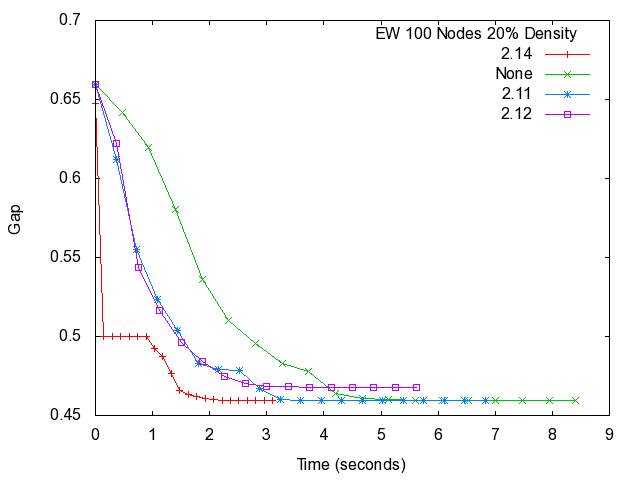
\includegraphics[width=0.6\textwidth]{plots/modelsgap-ew20-n100-sym.png}}
\subfloat[EW 100 Nodes 40\% Density]{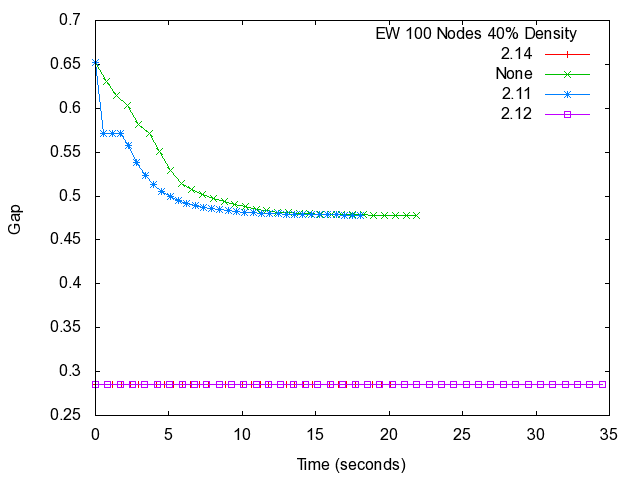
\includegraphics[width=0.6\textwidth]{plots/modelsgap-ew40-n100-sym.png}}
\\
\subfloat[EW 100 Nodes 60\% Density]{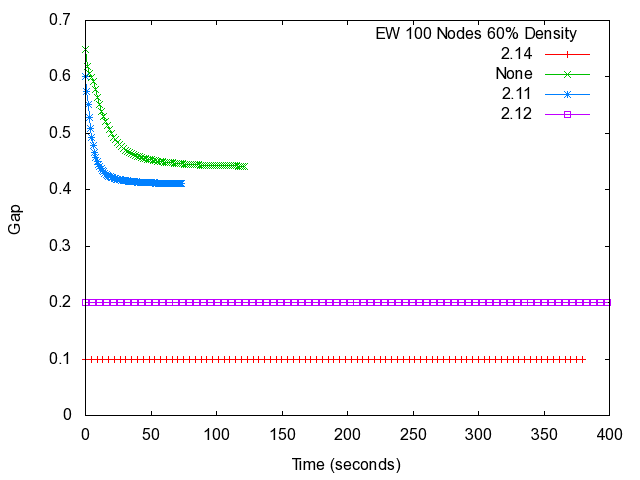
\includegraphics[width=0.6\textwidth]{plots/modelsgap-ew60-n100-sym.png}}
\subfloat[EW 100 Nodes 80\% Density]{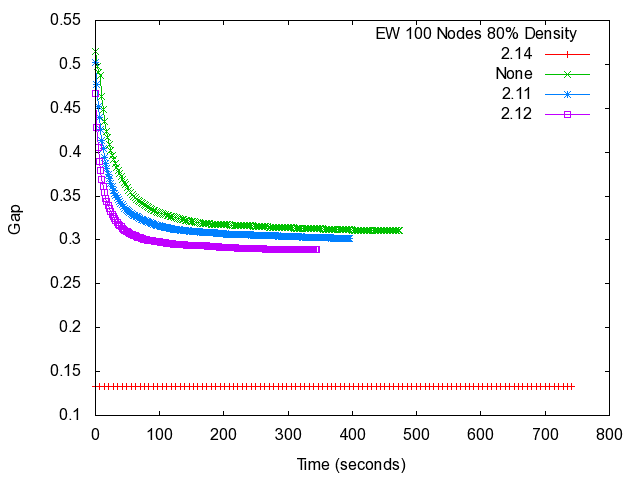
\includegraphics[width=0.6\textwidth]{plots/modelsgap-ew80-n100-sym.png}}
\caption{Comparison of the inclusion of different symmetry breaking constraints in the model, visualizing evolution of the gap during time in a cutting planes algorithm. Compared constraints are: assigning the lowest color label to the color class with the lowest node index \eqref{eqn:minlabel}, applying no constraint whatsoever, forcing lower labels to be used first \eqref{eqn:lowerlabel} and assigning the lowest color label to the color class with the greatest number of nodes \eqref{eqn:symnodecount}.}
\label{fig:models:sym}
\end{figure}


\subsubsection{Chosen formulation from cutting planes}
\label{subsubsec:results:model:chosen}

Taking into account all previous results in a cutting planes algorithm, the set of constraints that we will use in the \PCP{} formulation for subsequent computational experiments will be the following:

\begin{align}
\sum_{i \in P_k} \sum_{j \in C} x_{ij} = 1 \quad &\forall P_k \in P \tag{\ref{eqn:partsum}} \\
 \sum_{i \in N(i_0)} x_{i_0j} + r * x_{i_0j} \leq r * w_j \quad &\forall j \in C, \; \forall i_0 \in V \tag{\ref{eqn:adjsneighb}} \\
 w_j \leq \sum_{i \in V} x_{ij} \quad &\forall j \in C \tag{\ref{eqn:wjleqsumcolor}} \\
 x_{ij} \leq \sum_{l = j-1}^{k-1} \sum_{u \in P_l} x_{uj-1} \quad &\forall 1 < k \leq q, \; \forall i \in P_k, \; \forall 1 < j \leq k \tag{\ref{eqn:minlabel}} \\
 %w_j \geq w_{j+1} \sumheight \quad &\forall 1 \leq j < c \tag{\ref{eqn:lowerlabel}} \\
  x_{ij}, w_{j} \in \{0,1\} \quad &\forall i \in V, \; \forall j \in C \sumheight \nonumber
\end{align}

First two constraints define the problem itself, by specifying that a node must be colored in each partition and no color conflicts must occur; constraints \ref{eqn:wjleqsumcolor} simply strengthen the linear relaxation; and \ref{eqn:minlabel} eliminate symmetrical solutions. Last set of constraints are the binary restrictions.

Note that while adjacency restrictions \ref{eqn:adjscolorpone} reported better results than the chosen ones (\ref{eqn:adjsneighb}) in most cases, the latter worked better in dense graphs, which are the ones that, due to a larger problem size, take longer to solve their linear relaxation. Therefore, we opt for improving the resolution of the hardest graphs instead of getting slightly better results in the rest. 

\subsubsection{Branch and bound testing}

While the previous formulation was chosen for working on a cutting planes algorithm, we are also interested in the behaviour of different models in standard branch and bound algorithms. 

We tested many variations to the chosen model in a branch and bound algorithm, bound to $1800$ seconds, with graphs with $90$ nodes, partition size $2$ and different densities. The branch and bound uses default \textsc{cplex} settings, no custom callbacks were yet applied.

We present in table \ref{table:models:bnb} the following configurations, chosen based on their results:

\begin{itemize}
\defitem{M4}{Chosen model from cutting planes experimentation phase.}
\defitem{M1}{Relaxes that exactly one node must be painted per partition (\ref{eqn:partsum}) by replacing it with at least one painted per partition (\ref{eqn:partsumgeq}).}
\defitem{M8}{Strengthens the model using not only \ref{eqn:wjleqsumcolor} restrictions but also applying \ref{eqn:wjgeqsumpart}.}
\defitem{M3}{Uses simple color conflict constraints, requiring that two adjacent nodes cannot use the same color (\ref{eqn:adjscolorpone}).}
\defitem{M10}{Bases symmetry breaking on the number of nodes of each color class (\ref{eqn:symnodecount}).}
\end{itemize}

\begin{table}
\label{table:models:bnb}
\centering

\begin{tabular}{|c|c|c|c|c|}
\hline
\multicolumn{1}{|c|}{Id} & \multicolumn{1}{|c|}{M4} & \multicolumn{1}{|c|}{M1} & \multicolumn{1}{|c|}{M3}  & \multicolumn{1}{|c|}{M8} 
\\
\hline
EW 20 N=90 & \textbf{0.00} & \textbf{0.00} & 0.25  & \textbf{0.00}  
\\
EW 40 N=90 & 0.33 & \textbf{0.22} & 0.33 & 0.33 
\\
EW 60 N=90 & 0.39 & \textbf{0.37} & 0.41 & \textbf{0.37}
\\
EW 80 N=90 & 0.38 & 0.43 & \textbf{0.31} & 0.39
\\
\hline 
 \end{tabular}

\caption{Gap obtained in a standard branch and bound algorithm for different models.}

\end{table}

Results were most interesting. The formulation chosen for the cutting planes algorithm yielded good results only for lowest density graphs. In other cases, using different models returned better results:
\begin{itemize}
\item In graphs with $40\%$ density, relaxing the \ref{eqn:partsum} constraint on painting one node per partition greatly reduces the obtained gap, as can be seen in the results for $M1$.
\item In the most dense graphs, using tighter model strengthening constraints yields better results, as $M8$ has a much lower gap than the chosen model.
\item In the highest density graphs, using simple color conflict constraints returned a better result.
\end{itemize}

Although we will be using the previous formulation for fixing different settings throughout the following experimentations, we will reuse the results exposed here as alternative models for the final branch and cut algorithm, in order to pick the best performing model for the final version of the algorithm.

\clearpage